\section{Page-Wootters model: \texttt{NN}-level clock $+$ $2$-level system}

\begin{lstlisting}
NN := 32
\end{lstlisting}

\begin{lstlisting}
T := DiagonalMatrix[Range[0,NN-1]]
\end{lstlisting}

\begin{lstlisting}
F := FourierMatrix[NN]
\end{lstlisting}

For simplicity, $\hbar = 1$, there's no ``characteristic frequency'' $\omega$,
and we ignore the dimensional term in front of \eqref{eq:SI_Fourier:T}:

\begin{lstlisting}
\[CapitalOmega] := F.T.F\[ConjugateTranspose] 
\end{lstlisting}

Hamiltonian in "ordinary" space
\begin{lstlisting}
Hs := \[ImaginaryI]{{0, 1},{-1, 0}}
\end{lstlisting}
\begin{lstlisting}
MatrixForm[Hs]
\end{lstlisting}
\[
  \left(
    \begin{array}{cc}
     0 & i \\
     -i & 0 \\
    \end{array}
    \right)
\]

Matrix representation of \cite[Eq. 1]{Lloyd:Time}.
We turn it into numeric (\verb!N[ ]!) as treating  it symbolically onwards would be unfeasible:
\begin{lstlisting}
J := N[KroneckerProduct[\[CapitalOmega],IdentityMatrix[2]] + KroneckerProduct[IdentityMatrix[NN],Hs]]
\end{lstlisting}
\begin{lstlisting}
Chop[Eigenvalues[J]]

Out[ ] = {32., 31., 30., 30., 29., 29., 28., 28., 27., 27., 26., 26., 25., 25., 24., 24., 23., 23., 22., 22., 21., 21., 20., 20., 19., 19., 18., 18., 17., 17., 16., 16., 15., 15., 14., 14., 13., 13., 12., 12., 11., 11., 10., 10., 9., 9., 8., 8., 7., 7., 6., 6., 5., 5., 4., 4., 3., 3., 2., 2., 1., 1., -1., 0}
\end{lstlisting}
\begin{lstlisting}
Eigenvalues[J][[40]]

Out[ ] = 12.

Eigenvalues[J][[41]]

Out[ ] = 11.

chosenEigenvector := Eigenvectors[J][[ 40]]

chosenEigenvectorB := Eigenvectors[J][[41]]

Normalization := Sqrt[Abs[chosenEigenvector[[1]]^2] + Abs[chosenEigenvector[[2]]^2] ]

NormalizationB := Sqrt[Abs[chosenEigenvectorB[[1]]^2] + Abs[chosenEigenvectorB[[2]]^2] ]

chosenEigenvectorNormalized  := chosenEigenvector / Normalization

chosenEigenvectorNormalizedB := chosenEigenvectorB / NormalizationB  

probability := Abs[chosenEigenvectorNormalized ^2]

probabilityB := Abs[chosenEigenvectorNormalizedB^2]

probability

Out[ ]= {0.716702, 0.283298, 0.771924, 0.228076, 0.785749, 0.214251, 0.756071, 0.243929, 0.687408, 0.312592, 0.590214, 0.409786, 0.479286, 0.520714, 0.371512, 0.628488, 0.283298, 0.716702, 0.228076, 0.771924, 0.214251, 0.785749, 0.243929, 0.756071, 0.312592, 0.687408, 0.409786, 0.590214, 0.520714, 0.479286, 0.628488, 0.371512, 0.716702, 0.283298, 0.771924, 0.228076, 0.785749, 0.214251, 0.756071, 0.243929, 0.687408, 0.312592, 0.590214, 0.409786, 0.479286, 0.520714, 0.371512, 0.628488, 0.283298, 0.716702, 0.228076, 0.771924, 0.214251, 0.785749, 0.243929, 0.756071, 0.312592, 0.687408, 0.409786, 0.590214, 0.520714, 0.479286, 0.628488, 0.371512}

probabilityB

Out[ ]= {0.881533, 0.118467, 0.744511, 0.255489, 0.570264, 0.429736, 0.38532, 0.61468, 0.217835, 0.782165, 0.0933066, 0.906693, 0.0306941, 0.969306, 0.0395291, 0.960471, 0.118467, 0.881533, 0.255489, 0.744511, 0.429736, 0.570264, 0.61468, 0.38532, 0.782165, 0.217835, 0.906693, 0.0933066, 0.969306, 0.0306941, 0.960471, 0.0395291, 0.881533, 0.118467, 0.744511, 0.255489, 0.570264, 0.429736, 0.38532, 0.61468, 0.217835, 0.782165, 0.0933066, 0.906693, 0.0306941, 0.969306, 0.0395291, 0.960471, 0.118467, 0.881533, 0.255489, 0.744511, 0.429736, 0.570264, 0.61468, 0.38532, 0.782165, 0.217835, 0.906693, 0.0933066, 0.969306, 0.0306941, 0.960471, 0.0395291}

ListPlot[probability, GridLines ->{Range[0,NN*2, 2], Range[0, 1, 0.1]}, ImageSize->Large]
\end{lstlisting}
\begin{figure}
  \centering
  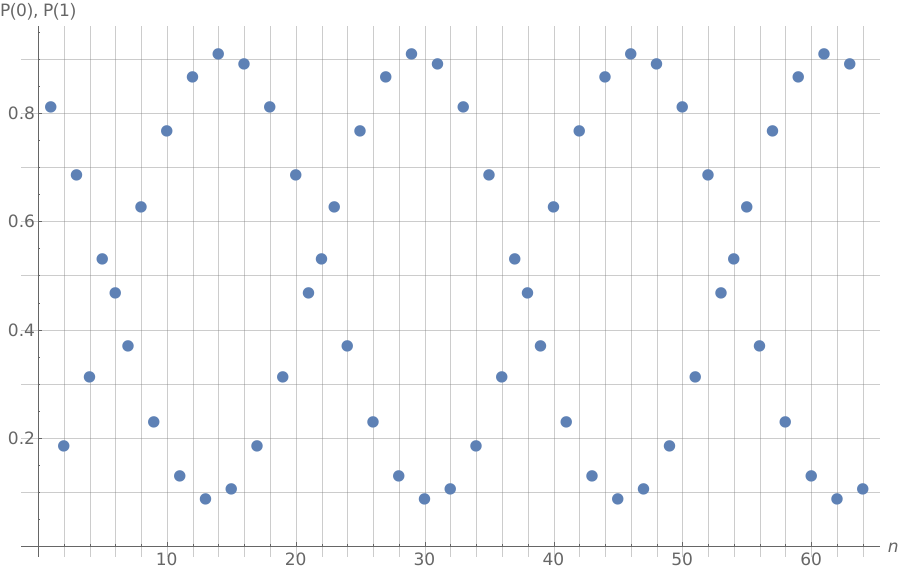
\includegraphics[width=0.75\textwidth]{img/N32.png}
  \caption[(from notebook)]{P-W ``evolution'' for $\hat{\mathbb{J}}$ eigenvalue $=12$}
  \end{figure}  
\begin{lstlisting}
ListPlot[probabilityB, GridLines ->{Range[0,NN*2, 2], Range[0, 1, 0.1]}, ImageSize->Large]
\end{lstlisting}
\begin{figure}
  \centering
  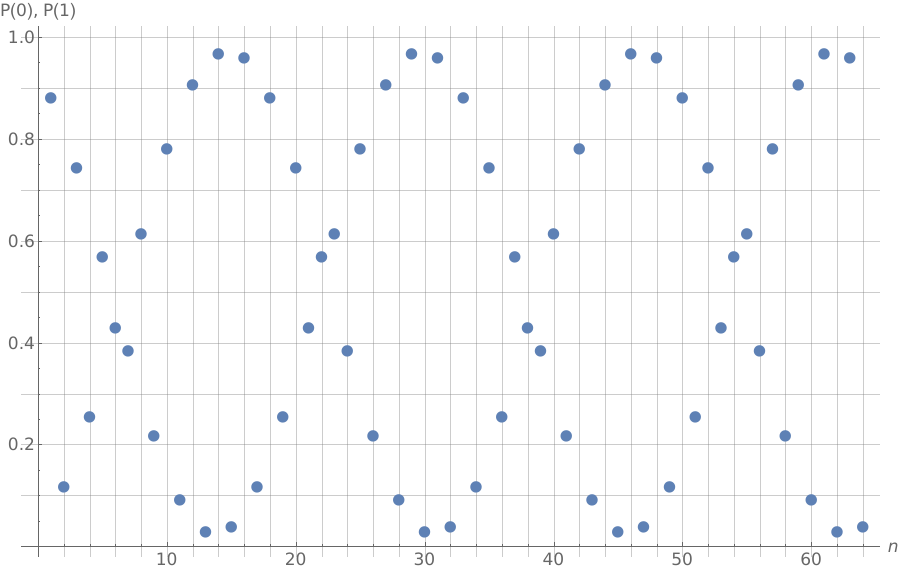
\includegraphics[width=0.75\textwidth]{img/N32-B.png}
  \caption[(from notebook)]{P-W ``evolution'' for $\hat{\mathbb{J}}$ eigenvalue $=11$}
\end{figure}

\subsection{Consistency of PW with ordinary QM (discrete approximation)}

\begin{lstlisting}

chosenEigenvectorNormalizedB 

Out[ ] = {-0.938878+0.00640243 I, 0.299377 -0.169824 I, 0.501468 -0.702168 I,-0.125361+0.489667 I, 0.233524 +0.718144 I,-0.390559-0.526498 I,-0.585152-0.207164 I, 0.783971 +0.0083447 I, 0.401462 -0.23804 I,-0.531014+0.707241 I,-0.0818027+0.294304 I,-0.282503-0.909332 I,-0.0173053-0.174341 I, 0.934362 +0.310279 I,-1.25607*10^-15+0.198819 I,-0.792316+0.576807 I,-0.169824-0.299377 I,-0.00640243-0.938878 I, 0.489667 +0.125361 I, 0.702168 +0.501468 I,-0.526498+0.390559 I,-0.718144+0.233524 I, 0.0083447 -0.783971 I, 0.207164 -0.585152 I, 0.707241 +0.531014 I, 0.23804 +0.401462 I,-0.909332+0.282503 I,-0.294304-0.0818027 I, 0.310279 -0.934362 I, 0.174341 -0.0173053 I, 0.576807 +0.792316 I,-0.198819+5.49532*10^-16 I,-0.938878+0.00640243 I, 0.299377 -0.169824 I, 0.501468 -0.702168 I,-0.125361+0.489667 I, 0.233524 +0.718144 I,-0.390559-0.526498 I,-0.585152-0.207164 I, 0.783971 +0.0083447 I, 0.401462 -0.23804 I,-0.531014+0.707241 I,-0.0818027+0.294304 I,-0.282503-0.909332 I,-0.0173053-0.174341 I, 0.934362 +0.310279 I, 3.53271*10^-16+0.198819 I,-0.792316+0.576807 I,-0.169824-0.299377 I,-0.00640243-0.938878 I, 0.489667 +0.125361 I, 0.702168 +0.501468 I,-0.526498+0.390559 I,-0.718144+0.233524 I, 0.0083447 -0.783971 I, 0.207164 -0.585152 I, 0.707241 +0.531014 I, 0.23804 +0.401462 I,-0.909332+0.282503 I,-0.294304-0.0818027 I, 0.310279 -0.934362 I, 0.174341 -0.0173053 I, 0.576807 +0.792316 I,-0.198819+0. I}

Out = {-0.938878 + 0.00640243 I, 0.299377 - 0.169824 I}
\end{lstlisting}